%%%%%%%%%%%%%%%%%%%%%%%%%%%%%%%%%%%%%%%%%%%%%%%%%%%%%%%%%%%%%%%%%%%%%%%%%%%%%%%%
%2345678901234567890123456789012345678901234567890123456789012345678901234567890
%        1         2         3         4         5         6         7         8

\documentclass[letterpaper, 10 pt, conference]{ieeeconf}  % Comment this line out if you need a4paper

%\documentclass[a4paper, 10pt, conference]{ieeeconf}      % Use this line for a4 paper

\IEEEoverridecommandlockouts                              % This command is only needed if 
                                                          % you want to use the \thanks command

\overrideIEEEmargins                                      % Needed to meet printer requirements.

% See the \addtolength command later in the file to balance the column lengths
% on the last page of the document

% The following packages can be found on http:\\www.ctan.org
%\usepackage{graphics} % for pdf, bitmapped graphics files
%\usepackage{epsfig} % for postscript graphics files
%\usepackage{mathptmx} % assumes new font selection scheme installed
%\usepackage{times} % assumes new font selection scheme installed
%\usepackage{amsmath} % assumes amsmath package installed
%\usepackage{amssymb}  % assumes amsmath package installed
\usepackage{graphicx}
\usepackage[export]{adjustbox}
\usepackage{hyperref}
\graphicspath{ {images/} }


\title{\LARGE \bf
Marine Multi-robot Patrolling
}

\author{Pin-Wei Chen$^{1}$, Ni-Ching Lin$^{2}$ and Po-Sheng Ser$^{3}$ % <-this % stops a space
\thanks{*This work was supported by the Robotics Master Program in National Chiao Tung University, Taiwan}% <-this % stops a space
\thanks{$^{1}$Pin-Wei Chen, National Chiao Tung University, Taiwan.		{\tt\small ccpwearth@gmail.com}}%
}


\begin{document}



\maketitle
\thispagestyle{empty}
\pagestyle{empty}


\section{INTRODUCTION \& MOTIVATION}

Multi-robot patrolling is an potential idea, we can apply this project to surveillance, security, production line, etc. We realize that robot can help us with something routine and cycling, such as patrolling, especially in marine field, which hasn't been highly protected and patrolled routinely. As a result, we come up with this idea, trying to build a multi-robot patrolling system in marine, and also build this system in ROS and combine with duckietown.

\section{SYSTEM ARCHITECTURE \& EQUIPMENTS}

\subsection{SYSTEM ARCHITECTURE}

We will have lots of robots(duckieboats) and one master robot(Raspberry Pi3). The all robots and master are all connected to the same router, so that the master can communicate with each robot.

Each robots will detect the specific patrolling node, which we use apriltag as, and follow it. As long as the robot arrive the specific patrolling node, it will stop and wait for the order from the master. The master will tell the robot to go to the next patrolling node.

\subsection{EQUIPMENTS} 

The robot I use is design by ourself and made by 3D printer and laser cut, which size is about 40*30*30, the 3D model of it is in Fig.~\ref{figure:model}. The robot contain a stereo camera(Zed) and two motors. In addition, we use apriltags or some particular geometric figures as the patroll nodes Fig.~\ref{figure:map}. In software part, We use ROS kinetic and ubuntu 16.04 LTS as our develop enviroment.

\begin{figure}[h] % h means put this image here
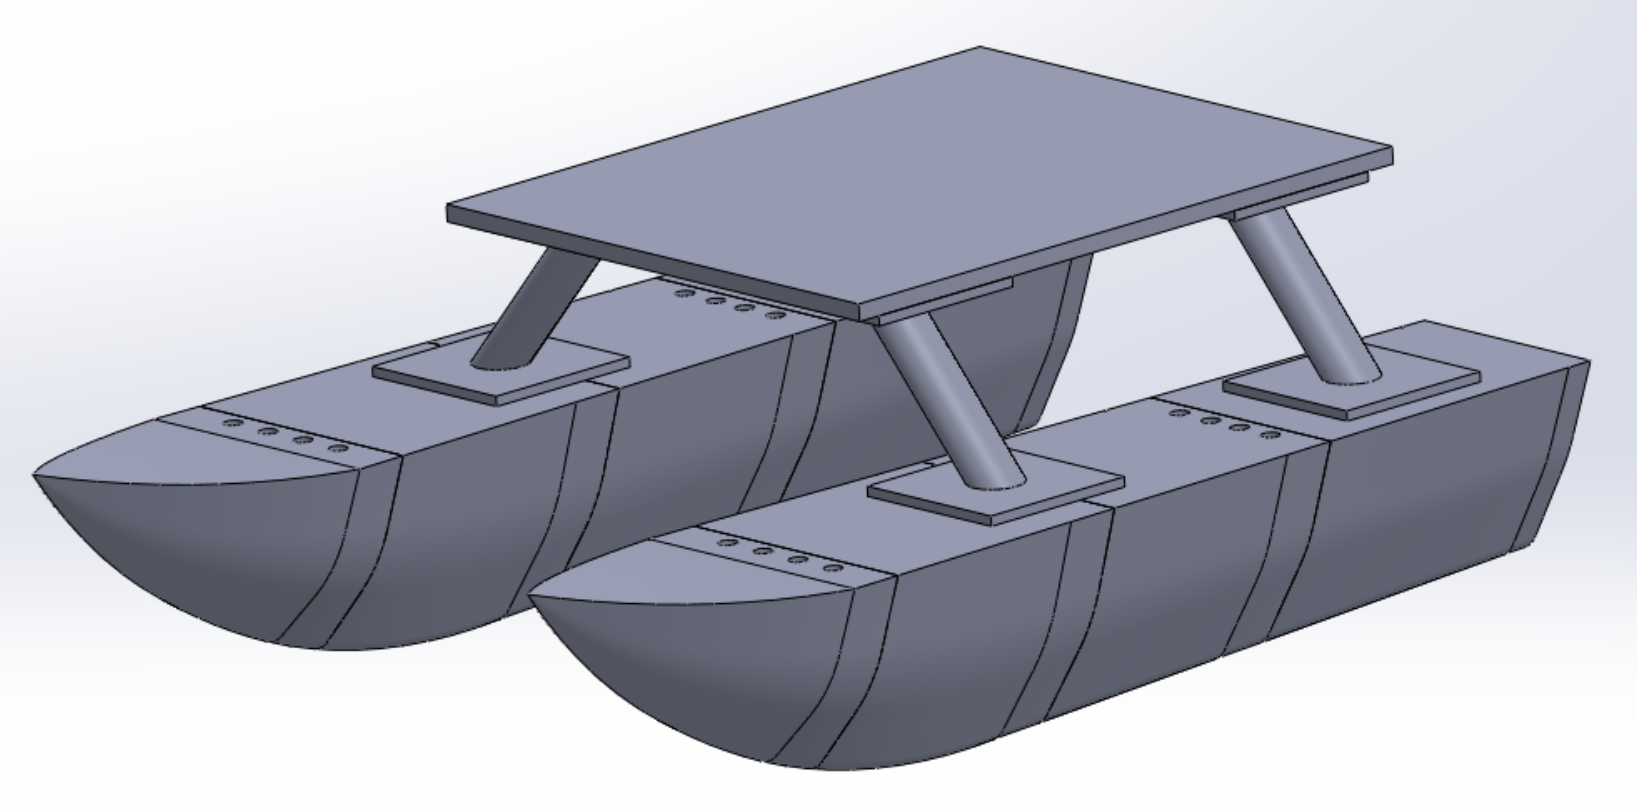
\includegraphics[width=0.9\columnwidth]{boat_model}
\centering
\caption{3D model of the boat}
 \label{figure:model}
\end{figure}

\begin{figure}[t] % t means put this image at the top 
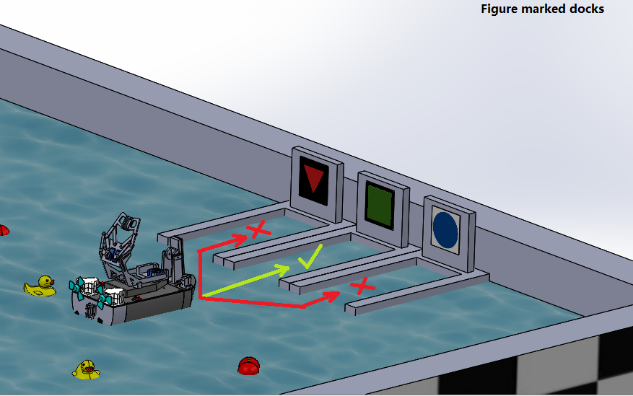
\includegraphics[width=0.9\columnwidth]{boat}
\centering
\caption{Marine robot}
\label{figure:map}
\end{figure}

\section{SPECIFIC AIMS}

\begin{itemize}
\item \textsl{Patrolling multi-node}
\end{itemize}
We are trying to let the robot patrol multi-node, and each node will be patrolled in approximately the same idle time. 
\begin{itemize}
\item  \textsl{Arrive specific patrolling node and avoid obstacles}
\end{itemize}
When the robot is going to visit specific patrolling node, and there are some obstacles floating between the robot and the goal, the robot should detect where the obstacles are and automatically avoid it.
\begin{itemize}
\item  \textsl{Multi-robot patolling}
\end{itemize}
We will let multi-robot patrol multi-node, in addition to each node will have same idleness, those robot will not patol on the same lane at the same time, or they will crash with each other.

\section{APPROACH}

We will use apriltags with different ID and some specific geometric figures to let the robot know which node they are patrolling now, it's kind of locate the robots.

The algorithm I use is refer to "Distributed On-line Dynamic Task Assignment for Multi-robot Patrolling"~\cite{Farinelli:2017:DOD:3124264.3124274}, we will measure the idleness of each node first, and than the master robot will coordinate every robot to let the nodes with large idleness be patrolled first. If any node is going to be patrolled, the idleness will return to zero, so that no two robots will go to the same node at the same time, and it can avoid collision.   


\section{SCHEDULE AND TEAM COLLABORATION}

I expect this project can complete patrolling system algorithm on land before November, and can do simple apriltag tracking in water before the end of December. The whole Marine Multi-robot Patrolling system can execute before the end of January, 2018. The experiment video is available in this link: \url{https://goo.gl/sDwa9j}

\addtolength{\textheight}{-12cm}   % This command serves to balance the column lengths
                                  % on the last page of the document manually. It shortens
                                  % the textheight of the last page by a suitable amount.
                                  % This command does not take effect until the next page
                                  % so it should come on the page before the last. Make
                                  % sure that you do not shorten the textheight too much.

\bibliographystyle{IEEEtran}
\bibliography{egbib}

\end{document}
